\chapter{电力系统脆弱性指标分析与综合评价模型}
\label{cha:quanti}

\section{引言}
\label{sec:index4}
在上一章中,通过对电力系统脆弱性的本质及脆弱过程进行研究分析,将电力系统的脆弱性分为结构脆弱性和状态脆弱性两个方面。结构脆弱性侧重于某一单元或某些单元退出后,
系统受影响的程度,考察的是某个单元在网络拓扑中的影响程度;状态脆弱性专注于系统的元件在扰动作用下,元件运行状态偏离正常状态的程度,考察的是系统的抗干扰能力。

为了对电力系统的脆弱性进行量化评估,得到脆弱性量化评估结果,基于上一章对结构和状态脆弱性指标的研究分析,分别针对结构脆弱性和状态脆弱性进行脆弱性评价指标的选取,
本章的研究重点在于脆弱性指标选取和多指标融合,建立系统脆弱性量化评估模型,进一步解决系统脆弱性系统脆弱性难以量化的问题,为下一章分析电力系统脆弱性问题,识别系统
脆弱环节奠定了理论基础。

\section{系统脆弱性量化评估指标}
\label{sec:describIndex}
为综合评价系统在扰动后所表现出的脆弱性,建立系统的量化评估模型,需要选取客观合理的系统脆弱性评判指标,并对指标进行分析描述,形成系统脆弱性综合评估指标集结构。



\subsection{电力系统的脆弱性指标选取}
\label{sec:pickIndex}
根据第三章对电力系统脆弱性的研究,将系统的脆弱性分为结构脆弱性和状态脆弱性。因此,本章将从这两个方面分别选取相应的系统脆弱性量化评价指标。

$(1)$结构脆弱性指标$I_1$:

对于结构脆弱性的评价来说,考察的是某一节点或线路因故障退出后对系统结构完整性的影响程度。对于系统结构影响程度大的节点或线路,说明其对网络拓扑结构的完整性贡献程度高,
对于这样的节点或线路称为系统结构的脆弱点。因此我们选取以下指标:

结构指标1:

在复杂网络理论中,度是网络特征的关键参数,描述的是节点的连接情况,表现出节点在结构拓扑中的重要程度。为评估系统节点在结构拓扑中的重要程度,选取电气度作为结构
脆弱性指标:$I_{11} = e_{i}$。

结构指标2:

基于复杂网络理论将系统拓扑等效为一个无向图,在描述网络特征的参数中,介数作为关键参数之一,被描述节点或边在信息、能量传递中的重要程度。为评估系统拓扑在能量传输分
布中的贡献,第二个结构脆弱性指标选为电气介数:$I_{12} = C_B(k)$。

结构指标3:

基于复杂网络理论中的$PageRank$算法,将结构拓扑中的支路潮流方向视为有向图,描述了节点之间的连接关系在系统拓扑的能量传递中的影响程度。第三个结构脆弱性指标选为$PR$值:
$I_{13} = PR(p_i)$。

$(2)$状态脆弱性指标$I_2$:

对于状态脆弱性的评价来说,考察的是在扰动作用下系统节点维持在稳定运行状态的能力,即系统抗干扰的能力,系统节点节点越容易到达临界失稳状态,说明节点的脆弱程度越高。
为了描述系统的当前状态与临界失稳状态的偏离程度,我们选取以下指标:

状态指标1:

电压作为评价电力系统安全稳定运行的重要指标。在电力系统运行过程中,通过比较节点实际的运行电压和临界电压之间的裕度来评估电网各节点的状态脆弱性,因此选取“电压裕度”指标
作为第一个状态脆弱性指标,考虑在概率负荷模型的情况下,基于蒙特卡洛模拟潮流计算的方法对电压裕度指标进行计算:$I_{21} = S_V$。

状态指标2:

通过上一章的状态脆弱性指标研究,通过连续潮流(CPF)计算各节点的临界负荷功率,该指标可以衡量节点所能承受的最大负荷能力,这有利于对负荷进行合理的规划分配。因此,选取
“功率稳定裕度”指标作为第二个状态脆弱性指标:$I_{22} = S_C$

状态指标3:

在电力系统脆弱性研究中,电力系统损耗也是需要重点考虑的一个方面,因此,选取“电网损耗灵敏度”指标第三个状态脆弱性指标:$$I_{23} = S_P = \frac{d P_{LOSS}}{d P_i}$$



\subsection{脆弱性量化评估指标的分析描述}
\label{sec:wordIndex}
电力系统结构脆弱性指的是电网在扰动作用下,保持其连通性和拓扑结构完整性的能力。其结构脆弱性指标描述的是节点在电力系统中的重要程度,本文认为对网络拓扑的完整性和连通性
贡献程度越高的节点,其脆弱程度越高,对电力系统的影响程度也越大。

$(1)$电气度指标:描述的是电力系统的连接情况和连接强度,表征的是系统节点在电力系统拓扑结构中的重要程度。电气度指标的计算是根据电力系统的节点的邻接矩阵和支路的视在功率
得出的,因此,系统节点的电气度指标越大,表示节点在此系统的重要程度越大,其脆弱程度越高。

$(2)$电气介数指标:描述的是电力系统各节点在能量传输分布中的贡献程度。电气介数指标越大,表示节点在能量传输中的贡献程度越高,其在意外扰动下退出时,对系统结构完整性的冲击
较大,其脆弱程度越高。

$(3)$PageRank值指标:PageRank值是基于$PageRank$互联网重要程度排序算法将电力系统等效为无权有向图得到的结构脆弱性指标,具体表现各节点在电力系统潮流传输方向上的能量累计。在潮流累计
分布中贡献程度高的节点,节点PageRank值越大,说明节点脆弱性越高。

电力系统状态脆弱性指的是系统在外界扰动或内部故障后,节点或支路的状态量向临界值逼近的特性。本文认为,在扰动作用下,电力系统中的节点或线路的运行状态值越接近临界失稳值,
其脆弱程度越大,越易影响系统的正常运行。

$(1)$电压裕度指标:电压是衡量电能质量的重要指标,在电力系统运行中,保证系统节点电压的稳定可以有效提高电力系统的运行效率,降低系统出现级联故障的可能性。在电压裕度指标的
计算中,我国规定。300$KV$及以上的母线,正常运行电压不得超过系统额定电压的10$\%$,因此电压偏差率取10$\%$,基于负荷功率模型的基础上,通过蒙特卡洛模拟试验方法,考察在负荷
变化的情况下,系统节点电压状态量的变化。通过电压裕度表达式可知,电压裕度指标值越小,其电压值越接近临界电压值,系统节点的脆弱程度越大。

$(2)$功率稳定裕度指标:描述的是系统节点所能承受的最大负荷量。在电力调度方面有利于合理调配负载,防止系统节点因过载而导致的电网故障。在指标计算方面,本文采用连续潮流(CPF)
计算得到各节点的最大有功负荷功率,进而得到各节点有功功率稳定裕度指标值。

$(3)$电网损耗灵敏度指标:描述的是系统各节点分别在负荷变化下对电网整体损耗的影响程度。这有利于识别出导致电网损耗率较高的关键元件,对降低电网损耗率具有参考价值。在指标计算方面,
考虑的是各节点的有功功率在额定值的$\pm 10 \%$范围内,按指定步长增加负荷,经过不断的潮流计算得到电网整体损耗值,进而得到系统的电网损耗灵敏度。因此,系统节点的灵敏度值越大,
节点的负荷变化对电网损耗越大,对电网元件的损耗越大,进而影响电网的整体运行状态。

本文在指标值处理上,采用“效益型”指标,指标值愈大愈好,具体指的是系统节点的指标值愈大,对电力系统的重要程度愈大,其脆弱程度愈高。

\subsection{系统脆弱性评估指标集结构及融合方法}
\label{sec:IndexSys}
通过电力系统脆弱性指标的选取和分析描述,电力系统的脆弱性评估指标分为结构脆弱性指标和状态脆弱性指标,从两个方面为各自部分脆弱性量化评估的依据。在一级结构指标中有电气度、电气介数
和PR值三个二级结构指标;在一级状态指标中有电压裕度、功率稳定裕度和电网损号灵敏度三个二级状态指标。整体的脆弱性评估指标集结构如图\ref{fig:index}所示。

\begin{figure}[H] % use float package if you want it here
    \centering
    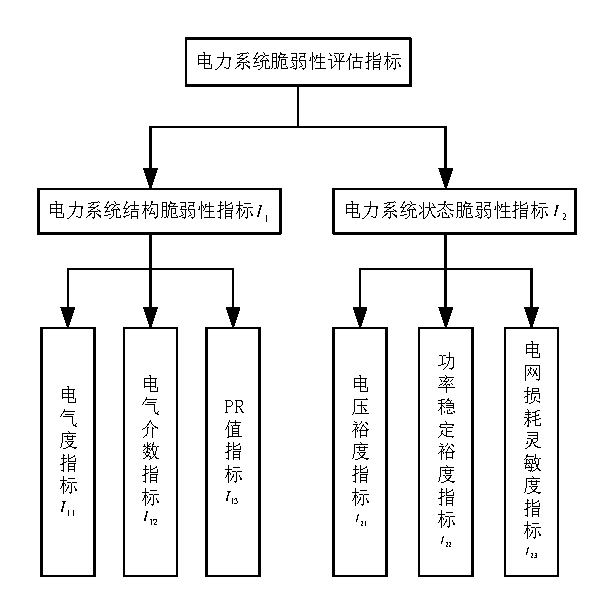
\includegraphics[]{index.pdf}
    \caption{电力系统脆弱性评估指标集}
    \label{fig:index}
  \end{figure}

针对多指标融合方法已有不少研究,在本文第一章绪论中,针对脆弱性评价指标建立系统评价模型的综述中提到,在指标融合方面,指标权重的确定方法主要分为主观法和客观法两类,主观法主要有专家调查法、
环比评分法、层次分析法等;而客观法主要有熵权法、基于方案满意度法 、基于方案贴近度法等。

主观赋权法是在权重分配方面研究较早、较为成熟的方法,其优点在于指标分析者可根据实际的决策问题和实际的知识经验合理地确定各指标的权重,避免出现权重分配结果与实际重要程度相悖的情况。但其缺点
也是相当明显,其评价结果具有较强的主观性,对指标分析者的水平要求较高,依赖于指标分析者的研究水平自身经验,同时增加了专家和决策分析者的研究负担,甚至出现决策偏差较大的情况,在实际应用中存在
很大的局限性。在主观赋权法中,层次分析法是应用最为成熟和广泛的赋权法之一,其在决策分析方法中的简洁实用、所需定量数据少的优点是使其广泛应用的主要原因。但其缺点也不能忽视,当指标过多时,对
决策者的科研水平和自身经验要求提高,主观成分过多,与此同时造成的数据统计量增大,权重难以确定,特征值和特征向量的精确求法也比较复杂。除此之外,根据检验对照表进行矩阵一致性检验,其权重确定
方法缺乏理论证明,其科学合理性不能充分令人信服。


客观赋权法是指单纯利用指标的客观信息而确定权重的方法,在结构脆弱性指标中,电气度、
电气介数和PageRank值这三个指标分别是从三个不同的方面进行研究提出的,对于研究分析者来说,无法从主观来判断其对评价结果的重要程度。另外,三个状态脆弱性指标也是分别从电压稳定性、最大负荷水平
和电网损耗三个角度来进行研究分析的,运用主观分析法进行权重分配,其方案的理论可信度不高,极有可能造成分配结果与实际情况不符,而客观赋权法其判断结果不依赖于人的主观判断,有较强的数学理论依据,
概念清楚,含义明确。

基于以上对主客观赋权法的分析,本文采用客观赋权的方法对电力系统结构和状态两个方面的脆弱性指标进行权重分配,仅根据各节点指标值的数据特点和分布进行权重分配,具有较强的数学理论支撑,不具有主观
随意性,可信度高。


\section{脆弱性量化评估二级指标融合方法研究}
\label{sec:processIndex}
从上述指标集结构来看,系统的二级指标是按照系统结构和状态划分的,从不同角度反映系统的脆弱性特征。针对所选取的结构和状态脆弱性评判指标,需要分别对其状态和结构脆弱性指标集进行融合,
首先要对各个二级指标进行归一化处理,消除量纲级的差异,选取并改进指标融合方法对指标进行权重分配,最后得到结构和状态一级评估指标。


\subsection{脆弱性量化评估指标数据归一化处理}
\label{sec:nomalzMethod}
针对基于不同理论和算法得出的脆弱性评估指标数据,不同指标数据在量纲和数量级上会存在差异。为了对系统节点进行脆弱性评估和指标融合,首先需要对指标数据进行归一化处理,数据的归一化方法
有很多,需要根据不同的数据格式和数据分布采取不同的归一化方法。下面对常用的归一化方法汇总如表\ref{tab:chap4:normalize}所示。
\begin{table}[H]
  \centering
  \caption{数据归一化方法汇总 }\label{tab:chap4:normalize}
  \begin{tabular}{C{3.8cm}C{2.9cm}C{2.7cm}C{3cm}}
  \toprule
  \textbf{方法} & \textbf{适用情况} & \textbf{特点} & \textbf{表达式}\\
        \midrule
        %\tabincell{c}{}
          \tabincell{c}{离差标准化\\(Min-max Normalization)}
           & 适用于最大最小值明确不变的数据      & 不改变数据的原始分布      & $x^{\ast}=\FS{x-x_{min}}{x_{max}-x_{min}}$   \\
  
         z-score~标准化       & 适用于最大值最小值未知的情况,且数据接近正态分布
                                          & 改变数据的原始分布,对离群点规范化效果好            & $x^{\ast}=\FS{x-\mu}{\sigma}$       \\
  
        Logistic~标准化       & 适用于对长尾分布的数据作分段操作
                                          & 改变数据的分布情况             & $x^{\ast}=\FS{\ln x}{\ln n_{max}}$       \\
  
        \tabincell{c}{小数定标标准化\\(Decimal scaling)}    & 适用于数据初期探索,不消除数据属性间权重差异
                                         & 不改变数据分布                      & $x^{\ast}=\FS{x}{10j}$       \\
  
        排序归一化             & 适用于对数据的具体值并不关心,更关心相对排序的数据
                                         & 原始数据变为直线分布            & $x^{\ast}=\FS{x_{rank}}{num_{total}}$       \\
  
        分段归一化             & 适用于数据分布有明显分段特征的情况
                                         & 不改变分段数据的分布            & 根据不同数据段,采用不用方法       \\
  \bottomrule
  \end{tabular}
  \end{table}

通过对数据归一化方法的整理与分析,针对指标集中的各项指标,采取合理的归一化方法将原始数据映射到$\left[0,1\right]$区间内,从而消除了数据之间的量纲和数量级的差异。

根据上节对量化评估脆弱性指标的分析描述,结构脆弱性的电气度、电气介数和PageRank值指标数据是根据复杂网络理论提出的,状态脆弱性的电压裕度、功率稳定裕度和电网损耗灵敏度指标
是根据裕度和灵敏度相关方法提出的,计算得到的指标数据其分布是可以真实反映各节点在系统中的重要程度。为了更好地衡量各节点在电网中的脆弱程度,不改变指标数值的原始分布。
本文在指标数据归一化处理上采用离差标准化方法。

采用离差标准化归一化方法时,需要明确知道数据的上限值和下限值,考虑到电气度、电气介数、PageRank值和电网损耗灵敏度指标无明确的上下限值,加之本文主要评估的是一个系统内各节点
的脆弱程度,所以本文选取同一指标下节点最大和最小指标值分别最为离差标准化的最大和最小值,这样不仅明确了数据的上下限,又不改变原始数据分布,真实反映各节点在系统中的重要程度。

归一化后的各节点的指标值均在$\left[0,1\right]$之间,因此得到归一化后的结构脆弱性指标向量$I_1$和状态脆弱性指标$I_2$。
\begin{equation}
  \left\{\begin{array}{l}{I_{1}=\left[\begin{array}{lll}{I_{11}^{*}} & {I_{12}^{*}} & {I_{13}^{*}}\end{array}\right]} \\
   {I_{2}=\left[\begin{array}{lll}{I_{21}^{*}} & {I_{22}^{*}} & {I_{23}^{*}}\end{array}\right]}\end{array}\right.
  \end{equation}

  
\subsection{基于改进熵权法的权重分配}
\label{sec:nomalz}
在复杂系统理论中,认为复杂系统具有异质性,复杂系统的异质性是指系统中各元件对整体影响程度的不均衡性。在电力系统中,各节点
对系统整体结构的影响程度体现在结构脆弱性指标值上,节点指标值越大,说明节点在系统结构拓扑中的重要性高,对系统整体的影响越大,其脆弱程度越高。
因此,本文认为,系统各节点的脆弱程度的差别是造成电力系统结构脆弱异质性的根本原因。
当系统各节点在某一指标下的指标值大致相近,说明各节点对系统的影响程度相近,进而无法分析各节点脆弱程度和识别系统脆弱环节,则该指标对综合
评价无参考价值。

熵作为热力学中分子运动无序程度的度量,原本用来反映系统蕴含能量的大小。随后被引入到各领域以表征系统无序程度。当分子均匀分布在整个空间内时,分析运动表现出高度的无序性特征,
系统的熵很大。当分子集中于系统中的某一子空间内时,分子运动无序程度很小,系统的熵很小\cite{refs76}。

在信息论中,熵是对信息量的一种描述。熵越大,包含的信息量越小;相反,熵越小,包含的信息量就越大。根据熵的特性,可以通过计算熵值来判断一个事件的随机性及无序程度,
也可以用熵值来描述指标间的差异程度,各指标值间的差别越大,该指标对综合评价的影响(权重)越大。

在结构脆弱性指标集中,每个评价指标是考虑不同节点对电网拓扑结构的影响程度而提出的,所以当指标的熵值越大,说明系统各节点对系统的影响程度比较均衡,
系统的异质性较小;反之,熵值越小,各节点的脆弱性差异也就比较大,系统具有较强的异质性。由于结构脆弱性各指标是从不同方面考虑提出的,不存在信息重合的情况。
所以在评价系统结构脆弱性指标时,基于熵权法的电网结构脆弱性特性分析与评价方法是比较合理的。

本文从熵的角度考虑,认为对于指标数据间差别较大的指标应赋予较高的权重。因此,在对结构脆弱性指标进行融合时,采用并改进熵权法对结构脆弱性指标进行权重分配。

下面对熵权法的步骤进行描述,并对数据处理过程中不合理之处进行改进。

首先,假设有$M$个评价对象,根据综合评估问题的需要,选取$N$个评价指标,计算各评价对象的各指标数值的大小,假设第$m$个评价对象的第$n$个评价指标数值为$\lambda_{mn}$。

然后,由于不同的评价指标在计算结果上存在量纲以及取值范围的差异,所以需要对每个评价指标的数值进行标准归一化处理。其归一化的数值用$\mu_{mn}$表示。

计算各评价指标的熵,表达式如下:
\begin{equation}
\label{equ:chap4:shang1}
  p_{m n}=\frac{\mu_{m}}{\sum_{m=1}^{M} \mu_{m}}
  \end{equation}

\begin{equation}
  H_{n}=-\frac{1}{\ln M} \sum_{m=1}^{M}\left(p_{m n} \ln p_{m n}\right)
  \end{equation}

式\ref{equ:chap4:shang1}中,$p_{mn}$表示第$n$组随机实验中第$m$个随机事件发生的概率(我们假设一个节点对应的指标值越大,其受到扰动或破坏的概率越大);$H_n$表示第$n$个指标的熵。

计算各评价指标的熵权,表达式如下:
\begin{equation}
  w_{n}=\frac{1-H_{n}}{\sum_{n=1}^{N}\left(1-H_{n}\right)}
  \end{equation}

具体映射:在电力系统结构脆弱性评估中,评价对象$M=39$,即1--39节点,评价指标$N=3$,分别为电气度、电气介数和PageRank值,将每个评价指标的数值在评价指标数值总和下所占的比例作为
其所发生的概率$p_{mn}$。

\begin{table}[htb]
  \centering
  \caption{熵权法与电力系统参数映射关系}
  \label{tab:lichaTable1}
    \begin{tabular}{C{5.5cm}C{5.5cm}}
      \toprule
      熵权法参数 & 电力系统参数 \\
      \midrule
      评价对象 &  系统节点 \\
      评价指标 &  结构脆弱性指标 \\
      评价对象概率值 & 节点的指标值占指标总和的比重 \\
      \bottomrule
    \end{tabular}
\end{table}

熵权法的计算流程如图\ref{fig:shang_Procession}所示:
\begin{figure}[H] % use float package if you want it here
  \centering
  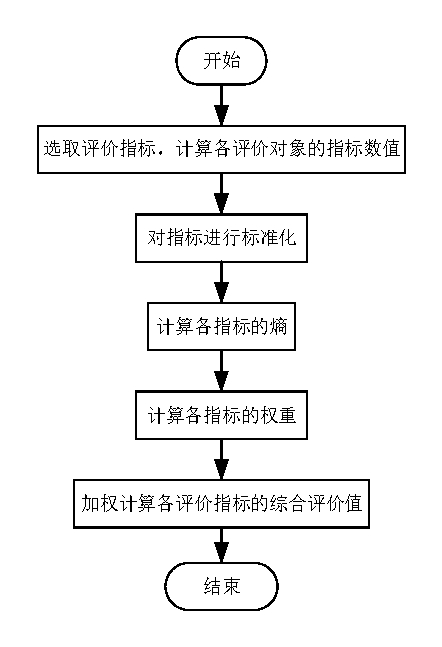
\includegraphics[]{shang_Procession.pdf}
  \caption{熵权法计算流程图}
  \label{fig:shang_Procession}
\end{figure}

在对指标数据进行归一化后,不可避免会出现数值为0的指标值,而熵权法赋权要求指标数据必须全部大于零,否则在取对数计算信息值时,会出现信息值异常的情况。针对这种情况,
传统熵权法的处理方法为:当$p_{mn}=0$,信息值$p_{m n} \ln p_{m n}=0$。这说明脆弱指标值为0的系统节点,其在脆弱程度评价所提供的信息为0,对脆弱性综合评价不起作用。
而在实际的电力系统脆弱性分析中,虽然有的节点在某一脆弱性指标下的指标值极小,但实际却在电网结构和运行中承担极大的作用。其次,其$p_{mn}=0$的信息值与$p_{mn}=1$的
信息值相等,因此,在电网脆弱性指标权重分配处理上,这种方法是不合理的。

为此,考虑到电力系统节点的潜在脆弱性特征,避免在数据处理过程中出现异常,保证数据的完整性和评价的可靠性。本文在不改变指标数据的原始分布的前提下,将结构脆弱性指标归一化
到$[0.002,0.998]$区间内。在对指标数据进行变换后,现有数据会与原始数据有所偏差,本文将其定义为信息损失,除此之外,本文还将对信息损失进行度量,比较指标数据变换前后各指
标数据与均值的偏离程度来量化信息损失,即用方差来定义
信息损失度$\beta$:
\begin{equation}
  \label{equ:chap4:infoloss}
\sum_{i=1}^{n}\left(\mu_{i}^{*}-\bar{\mu}_{i}^{*}\right)^{2} /\sum_{i=1}^{n}\left(\mu_{i}-\bar{\mu}_{i}\right)^{2} \geq 1-\beta 
\end{equation}

式\ref{equ:chap4:infoloss}中,称$\mu_{i}^{*}$为在信息损失度为$\beta$下的指标数据,$\mu_{i}$为原始指标数据。

根据上述改进熵权法,可计算得到在信息损失度为$\beta=0。008$下的结构脆弱性评价指标的权重向量$W$为:
\begin{equation}
\label{equ:chap4:shang2}
   W_1 = \left[w_{1}\ w_{2}\ w_{3}\right]=[0.33\ 0.41\ 0.26]
\end{equation}



\subsection{基于离差最大化法的权重分配}
\label{sec:nomalz}
在状态脆弱性指标研究方面,本文从节点电压稳定性、节点最大负荷功率和电网损耗方面考虑分别提出了电压裕度、功率稳定裕度和电网损耗灵敏度指标来进行电力系统状态脆弱性研究。
在状态脆弱性指标的权重确定方面,本文认为在某一状态指标下,电网各节点的状态指标值是不同的,当电力系统各节点的状态指标值的差别很小时,说明选取的指标在电力系统的量化评估中起到的
作用很小,应赋予小的权重,这在一定程度反映一个问题,这就是为什么我们在选取评价指标时,要从不同方面考虑,做的全面客观地选取指标。当电力系统各节点的状态指标值离散程度
大时,说明选取的指标使各节点的状态值产生了很大的变化,不同节点在此指标下的状态值差别很大,说明选取的指标在电力系统的量化评估中起到的作用很大,应赋予较大的权重。

本文将状态脆弱性指标权重分配的问题与多属性决策相联系,采用在多属性决策领域常用权重分配方法--离差最大化法进行状态指标的权重分配,离差最大化的基本思想,量化描述在指标$i$下,
各方案的指标值的离散程度,其表征的意义在于,如果指标$i$对于所有的方案而言,各方案的指标值$u_{ij}$均无差别,那么指标$i$对方案决策与排序将不起作用,这样的评价指标可令其权重系数为0;
如果$i$ 指标能使决策方案的指标值$u_{ij}$间的有较大差异,这样的评价指标对方案决策与排序将起重要作用应该给予较大的权重系数\cite{refs77,refs78}。

通过上述的分析可知,本文认为在电力系统状态脆弱性评估方面,在某一指标下,若系统节点间的状态指标值差别很大,说明该指标在电力系统状态评估方面起到很大的作用,应赋予较大的权重。
因此,在状态脆弱性指标融合方面,本文选用离差最大化法对状态脆弱性指标进行权重分配。

在多属性决策方面,对于某个多属性决策问题,设其方案集为$A = \{A_1,A_2 \cdots A_m\}$,属性集为$G = \{G_1,G_2 \cdots G_n\}$,方案$A_i$对属性$G_j$的指标值
记为$y_{ij}\left(i = 1,2,\cdots,m;j = 1,2,\cdots,n\right)$,矩阵$Y = \left(y_{ij}\right)_{m \times n}$表示方案集A对属性集G的“属性矩阵”,俗称“决策矩阵”。
% 通常指标的类型有“效益型”指标、“成本型”指标、“固定型”指标和“区间型”指标。“效益性”指标是指属性值愈大愈好的指标,如资金产值率、人均国民生产总值等;“成本型”指标是指属性值愈
% 小愈好的指标,如流动资金占用额,资金周转天数等;“固定型”指标是指属性值既不能太大又不能太小,而以稳定在某个固定值为最佳的一类指标,家用电器稳压器的稳压性能指标就属于
% 这类指标;“区间型”指标是指属性值以落在某个固定区间内为最佳的一类指标,国家标准中规定的等级划分通常都属于这类指标。
在4.2.2节的脆弱性量化评估指标的分析描述中,本文在指标处理上采用的“效益型”指标,指标值越大越好\cite{refs78}。

对矩阵$Y$进行归一化处理后得到的决策矩阵记为$Z = (z_{ij})_(m \times n)$,显然,$z_{ij}$愈大愈好,设评价指标间的加权向量为$W = [w_1,w_2 \cdots w_n]^T > 0$,并满足
单位化约束条件
\begin{equation}
  \sum_{j=1}^{m} w_{j}^{2}=1
\end{equation}
  
在加权向量$W$的作用下,构造加权规范化决策矩阵
\begin{equation}
C = \left[\begin{array}{cccc}{w_{1} z_{11}} & {w_{2} z_{12}} & {\cdots} & {w_{n} z_{1 n}} \\ {w_{1} z_{21}} & {w_{2} z_{22}} & {\cdots} & {w_{n} z_{2 n}} \\ 
{\vdots} & {\vdots} & {} & {\vdots} \\ {w_{1} z_{m 1}} & {w_{2} z_{m 2}} & {\cdots} & {w_{n} z_{m n}}\end{array}\right]
\end{equation}

根据简单加性加权法(SAW),各决策方案$A_i$的多指标综合评价值可表示为
\begin{equation}
\label{equ:chap4:SAW}
  D_i(w) = \sum_{j = 1}^{n} z_{ij}w_{j} , i=1,2 \cdots n
\end{equation}

可以看出,$D_i(w)$值愈大表明决策方案$A_i$愈优。因此,在加权向量$W$已知的情况下,根据式\ref{equ:chap4:SAW}可以对各决策方案进行决策或排序。下面将求解加权向量$W$.
根据离差最大化的基本思想,对于$G_j$属性而言,存在一组权重向量W,使得决策方案$A_{i}$与其他所有的决策方案的离差最大,其表达式可定义为
\begin{equation}
\begin{aligned} V_{i j}(w) &=\sum_{k=1}^{m}\left|w_{j} z_{i j}-w_{j} z_{k j}\right| \\ i=& 1,2 \cdots m, j=1,2 \cdots n \end{aligned}
\end{equation}

令
\begin{equation}
\begin{aligned} V_{j}(w)=\sum_{k=1}^{m} V_{i j}(w) &=\sum_{k}^{m} \sum_{k=1}^{m}\left|z_{i j}-z_{k j}\right| w_{j} \\ j=1,2 \cdots n \end{aligned}
\end{equation}

则$V_{j}(w)$表示对$G_{j}$而言,所有决策方案与其他决策方案的总离差。根据离差最大化的思想,加权向量$W$的确定应是总离差$V_{j}(w)$最大。为此,构造目标函数为
\begin{equation}
\label{equ:chap4:licha1}
\begin{aligned} \max F(w) &=\sum_{j=1}^{n} V_{j}(w) \\ &=\sum_{j=1}^{n} \sum_{i=1}^{m} \sum_{k=1}^{m}\left|z_{i j}-z_{k j}\right| w_{j} \end{aligned}
\end{equation}

于是,求解加权向量$W$转化为求解式\ref{equ:chap4:licha1}的最大值问题
\begin{equation}
\label{equ:chap4:lichaMode}
\left\{\begin{array}{l}{\max F(w)=\sum_{j=1}^{n} \sum_{i=1}^{m} \sum_{k=1}^{m}\left|z_{i j}-z_{k j}\right| w_{j}} \\ 
{\text { s.t. } \sum_{j=1}^{n} w_{j}^{2}=1}\end{array}\right.
\end{equation}

解此最优化模型\ref{equ:chap4:lichaMode},得到
\begin{equation}
  w_{j}=\frac{\sum_{k=1}^{m} \sum_{k=1}^{m}\left|z_{i j}-z_{i j}\right|}{\sum_{j=1}^{n}\left[\sum_{i=1}^{m} \sum_{k=1}^{m} | z_{ij}-z_{k j} | \right]^{2}}, j=1,2 \cdots n
  \end{equation}

理论上可以证明$W^* = [w_1,w_2 \cdots w_n]^T$为目标函数$F(w)$的唯一极大值点。 在得到单位化加权向量$W^*$后,为了进行权重分配,需要对$W^*$进行归一化处理
\begin{equation}
  \bar{w_{j}} = \frac{w_{j}^*}{\sum_{j=1}^{n} w_{j}^*} , j=1,2 \cdots n  
\end{equation}

由此得到归一化权重向量
\begin{equation}
  \bar{w_{j}}=\frac{\sum_{k=1}^{m} \sum_{k=1}^{m}\left|z_{i j}-z_{i j}\right|}{\sum_{j=1}^{n}\sum_{i=1}^{m} \sum_{k=1}^{m} | z_{ij}-z_{k j}|}, j=1,2 \cdots n
  \end{equation}

本文在运用离差最大化进行状态脆弱性指标融合时,方案集$A_i$对应系统节点名称,属性集$G_j$对应状态脆弱性指标集,方案的属性值对应为系统节点的指标值。其映射关系如表\ref{tab:lichaTable1}
所示:
\begin{table}[htb]
  \centering
  \caption{多属性决策与电力系统参数映射关系}
  \label{tab:lichaTable1}
    \begin{tabular}{C{4.5cm}C{4.5cm}}
      \toprule
      多属性决策参数 & 电力系统参数 \\
      \midrule
      方案集 & 系统节点集 \\
      属性集 & 状态脆弱性指标集 \\
      方案的属性值 & 系统节点的指标值 \\
      \bottomrule
    \end{tabular}
\end{table}

综上所述,运用离差最大化法对状态脆弱性指标进行权重分配的步骤如图\ref{fig:licha_Procession}下:
\begin{figure}[H] % use float package if you want it here
  \centering
  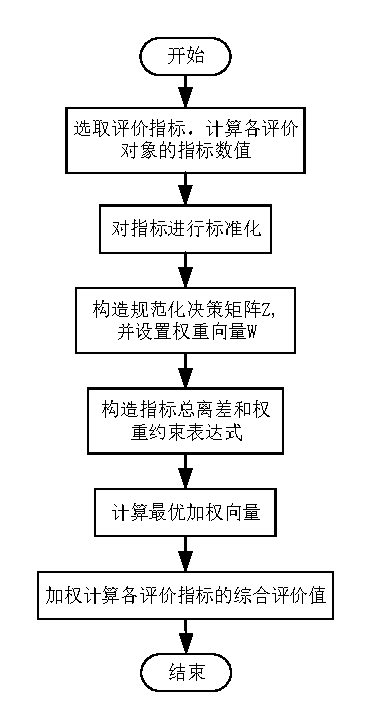
\includegraphics[]{licha_Procession.pdf}
  \caption{离差最大化权重分配流程图}
  \label{fig:licha_Procession}
\end{figure}

根据上述离差最大化原理,计算得到状态脆弱性指标集权重向量$W$如下:
\begin{equation}
  \label{equ:chap4:quanzhong2}
    W_2 = \left[w_{1}\ w_{2}\ w_{3}\right]=[0.29\ 0.34\ 0.37]
    \end{equation}


\subsection{脆弱性量化评估二级指标融合}
\label{sec:2ndIndexMerge}

通过第三章对电力系统脆弱性指标的研究和计算,得到脆弱性指标值后,运用$Matlab$工具实现对结构脆弱性指标和状态脆弱性指标的权重分配,其权重分配结果汇总如下:
\begin{table}[htb]
  \centering
  \caption{二级指标权重分配结果}
  \label{tab:quanzhong3}
    \begin{tabular}{C{3.5cm}C{3.5cm}C{3.5cm}}
      \toprule
      指标类型 & 指标名称 & 权重系数 \\
      \midrule
                    & 电气度  &  0.33 \\
      结构脆弱性指标 & 电气介数 & 0.41 \\
                    & PageRank值 & 0.26 \\
                    & 电压裕度  &  0.29 \\
      状态脆弱性指标 & 功率稳定裕度 & 0.34 \\
                    & 电网损耗灵敏度 & 0.37 \\ 
      \bottomrule
    \end{tabular}
\end{table}

\begin{figure}[H] % use float package if you want it here
  \centering
  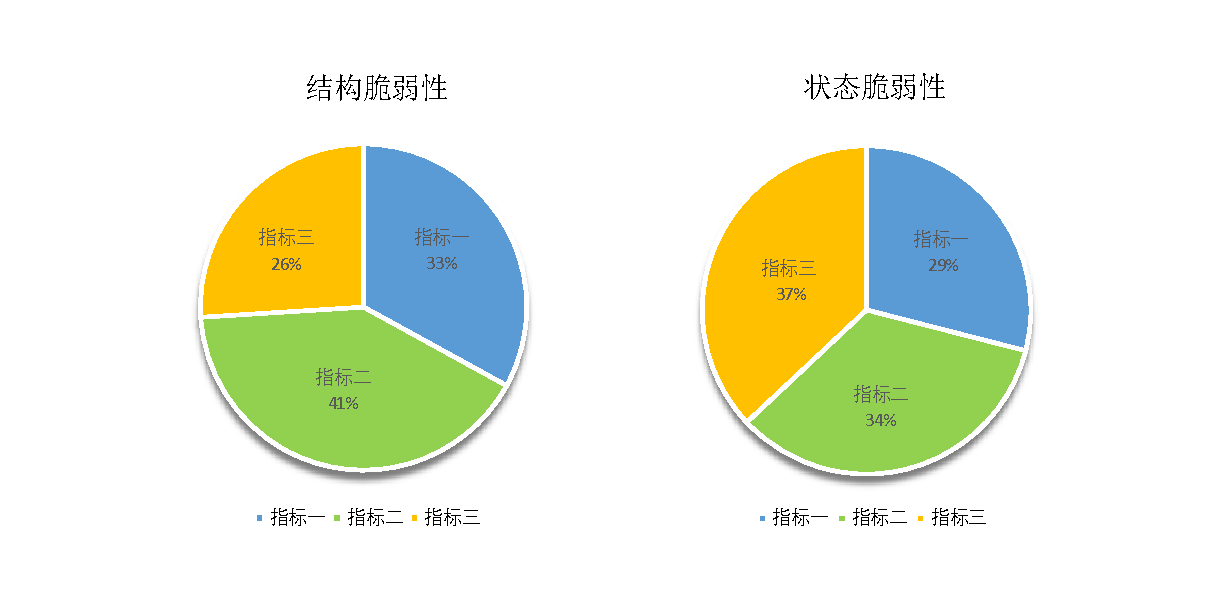
\includegraphics[width=14cm,height=7cm]{quanzhong.pdf}
  \caption{系统二级脆弱性指标权重图}
  \label{fig:quanzhong}
\end{figure}

从图\ref{fig:quanzhong}中可以看出,对于结构脆弱性指标而言,指标二电气介数对于电力系统脆弱性评价影响最大,因为该指标在进行节点重要性分析时,不仅考虑到系统节点在拓扑中的重要性
还考虑到潮流能量分布对结构的影响程度,所以从改进的熵权法的权重结果上,电气介数在脆弱性评估上赋予较大的权重是合理的。对于状态脆弱性指标而言,各指标的权重分配结果差别不大,其中
指标二功率稳定裕度和指标三电网损耗灵敏度所占权重较大,而指标一电压稳定裕度权重最小,其原因在于电力系统各节点的差异性,在指标二和指标三中,两个指标都是各自节点参数的改变来确定各
节点的指标值,如电网损耗灵敏度指标,该指标是通过增加某节点的有功功率经潮流计算得到电网损耗值。指标一不同的是,该指标是运用蒙特卡洛模拟实际电网负荷变化,来计算节点电压的平均电压裕度,
加之电网电压在实际负荷变化情况下,其本身的稳定性较强,电压值变化幅度较小,导致各节点的指标值离散程度较小,所以该指标在最大离差化法的权重计算结果中,所占的权重最小。

因此,本文由权重分配结果对结构和状态的各脆弱性指标进行融合,其表达式如下:
\begin{equation}
\begin{aligned} V_{1} &=I_{1} \cdot W_1^{T} \\ &=\left[\begin{array}{lll}{I_{11}^{*}} & {I_{12}^{*}} & {I_{13}^{*}}\end{array}\right] \cdot\left[\begin{array}{lll}{w_{1}} & {w_{2}} & {w_{3}}\end{array}\right]^{T}, V_{1} \in[0,1] \end{aligned}
\end{equation}
\begin{equation}
\begin{aligned} V_{2} &=I_{1} \cdot W_2^{T} \\ &=\left[\begin{array}{lll}{I_{21}^{*}} & {I_{22}^{*}} & {I_{23}^{*}}\end{array}\right] \cdot\left[\begin{array}{lll}{w_{1}} & {w_{2}} & {w_{3}}\end{array}\right]^{T}, V_{2} \in[0,1] \end{aligned}
\end{equation}


\section{脆弱性量化评估一级指标融合}
\label{sec:DS}
经过上节的研究分析得到了结构和状态两个独立的评判指标$V_1$和$V_2$,将这两个一级指标进行融合是本节研究的重点,本文用概率统计的方法对系统的脆弱程度进行评估,也就是将系统的脆弱性事件分为两类:
脆弱和非脆弱,考虑到事件和一级指标间的独立性,本节基于D-S证据理论,对一级指标进行融合,最终得到一个$0-1$范围内的系统脆弱性综合评价结果。

\subsection{D-S证据理论}
\label{sec:DStheory}
D-S证据理论是最早由Dempster提出,后由Shafter进行补充的用于处理不确定性问题的完整理论。其原理是Dempster通过定义命题的不确定性,提出集值映射和上、下限概率的概念,然后给出Dempster法则
作为证据融合规则,最后Shafer引入信任函数重新定义上、下限概率,得出具有普适性的D-S证据理论。D-S证据理论的特点:由贝叶斯理论发展而来,但约束条件比贝叶斯概率理论更弱;采用“区间估计”而非
“点估计”来描述事件的不确定性;不仅能够强调事物的客观性,还能强调人类对事物估计的主观性\cite{refs79}。

\begin{definition}
辨识框架(Frame of Discernment)
\end{definition}
设$\Theta=\left\{\theta_{1}, \theta_{2}, \ldots, \theta_{n}\right\}$,若非空集合$\Theta$是由$n$个互不相容的元素组成,那么称$\Theta$是辨识框架。

在D-S证据理论中,辨识框架表示关于命题的彼此独立的所有答案或假设的有限集合\cite{refs80}。$2^\Theta$是$\Theta$的幂集,表示辨识框架的所有子集(包含空集),
即$2^{\Theta}=\left\{\phi,\left\{\theta_{1}\right\},\left\{\theta_{2}\right\}, \ldots,\left\{\theta_{n}\right\},\left\{\theta_{1}, \theta_{2}\right\},\left\{\theta_{1}, \theta_{3}\right\}, \ldots, \Theta\right\}$。

\begin{definition}
基本概率赋值函数(Basic Probability Assignment)
\end{definition}
设$\Theta$为一识别框架,$A$是$\Theta$上的任意子集,若函数$m$:$2^{\Theta} \rightarrow[0,1]$,满足条件
\begin{equation}
\left\{\begin{array}{l}{m(\emptyset)=0} \\ {\sum_{A \subset \Theta} m(A)=1} \\ {m(A)>0}\end{array}\right.
\end{equation}

称函数$m$是$2^\Theta$上的概率赋值函数。$\forall A \subset \Theta$,$m(A)$为$A$的基本信任值,表示该条证据对命题$A$的支持程度,$m(A)$仅表示对$A$的信任,不反映对其他任何子集的支持度。
其中,使得$m(A)>0$的$A$称为焦元。
\begin{definition}
置信函数(Belief Function)和似真函数(Plausibility Function)
\end{definition}
\begin{equation}
  \operatorname{Bel}(A)=\sum_{B \subseteq A} m(B), \forall A \subseteq \Theta
\end{equation}
\begin{equation}
  \operatorname{Pl}(A)=\sum_{B \cap A \neq \varnothing} m(B)
\end{equation}

上式中,$B$为$A$的子集,函数$Bel$是$\Theta$上的置信函数。对于任一$A \subset \Theta$,$Bel(A)$是对$A$的置信度,表示$A$发生的可能性;函数$Pl$是辨识框架$\Theta$上的似真函数。
对于任一$A \subset \Theta$,$Pl(A)$是对$A$的似真度,表示$A$可能为真的不确定度量。在证据理论中,通常用$\left[Bel(A),Pl(A)\right]$来表示证据对$A$的信任区间。D-S证据理论对于事件A的
不确定性描述如图\ref{fig:undefined}所示。
\begin{figure}[H] % use float package if you want it here
  \centering
  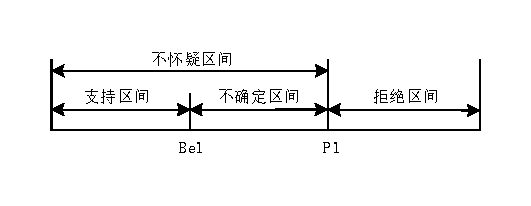
\includegraphics[]{undefined.pdf}
  \caption{对事件A的不确定性描述}
  \label{fig:undefined}
\end{figure}
\begin{table}[htb]
  \centering
  \caption{对命题A各区间的解释}
  \label{tab:undefined}
    \begin{tabular}{C{5.5cm}C{6cm}}
      \toprule
      $\left[Bel(A),Pl(A)\right]$ & 解释描述 \\
      \midrule
      $\left[0,1\right]$ & 对命题A完全不确定 \\
      $\left[0.7,0.7\right]$ & 命题A为真的准确概率为0.6 \\
      $\left[0,0\right]$ & 命题A完全为假 \\
      $\left[1,1\right]$ & 命题A完全为真 \\
      $\left[0.4,0.6\right]$ & 命题A为真的概率在0.4和0.6之间 \\
      \bottomrule
    \end{tabular}
\end{table}

在证据理论的合成规则上,假设$m_1,m_2,\cdots,m_k$分别是同一识别框架$\Theta$上的$k$个基本概率赋值函数,对应的焦元分别为$A_i(i=1,2,\cdots,k)$,设
$K=\sum_{A_{1} \cap \cdots \cap A_{k} = \varnothing } m_{1}\left(A_{1}\right) m_{2}\left(A_{2}\right) \cdots m_{k}\left(A_{k}\right)<1$,若映射$m$:
$2^ \Theta \rightarrow \left[0,1\right]$,则$k$条证据的合成规则为:
\begin{equation}
\label{equ:chap4:rules}
m(A)=\left\{\begin{array}{ll}{0} & {A=\Theta} \\ {\frac{\sum_{A_{1} \cap A_{2} \cap \cdots \cap A_{k}=A} m_{1}\left(A_{1}\right) m_{2}\left(A_{2}\right) \cdots m_{k}\left(A_{k}\right)}{1-K}} & {A \neq \Theta}\end{array}\right.
\end{equation}

式\ref{equ:chap4:rules}中,$K$表示证据间的冲突系数,表示证据间的冲突系数。

式\ref{equ:chap4:rules}融合公式需要满足两个条件\cite{refs81}:
\begin{itemize}
  \item 各证据间互不影响,数据信息相互独立。
  \item 辨识框架中各事件具有互斥性和完备性。 
\end{itemize}

通过研究可以得出,D-S证据理论中不确定性推理流程为:

$(1)$建立辨识框架$\Theta$,确定命题的完备集,生成基本概率赋值函数(BPA);

$(2)$对各证据进行组合,对加入的证据进行概率更新,计算冲突系数$K$;

$(3)$确定计算事件的$Bel$和$Pl$,得到事件置信区间;

$(4)$根据Dempster证据组合规则,计算确定事件的BPA函数;

$(5)$将BPA函数的可信度转换为概率,对融合结果做出决策。

\subsection{脆弱性量化评估一级指标融合}
\label{sec:DSdistri}
在本文中,电力系统脆弱性分结构和状态两方面进行研究,通过客观赋权融合方法分别得到结构指标$V_1$和状态指标$V_2$,这两个指标分别从两个完全不同的方面对系统脆弱性问题展开分析的,
因此,可将这两个一级指标视为两条独立的证据,它们分别从不同方面对系统脆弱性这一不确定性事件进行描述评估。鉴于D-S证据理论是用于处理不确定性问题的完备理论,所以对于电力系统脆弱性
的综合评价问题满足D-S证据理论的约束条件。

由上述分析可知,电力系统脆弱性辨识框架由两个事件构成完备事件集:脆弱和非脆弱。结构脆弱性指标和状态脆弱性指标可作为指向系统脆弱性的两条独立的证据,其中概率赋值函数(BPA)可用指标概率值$P$
表示:
\begin{equation}
\left\{\begin{array}{l}{ V_1 = P_1 \times 100\%} \\ {V_2 = P_2 \times 100\%}\end{array}\right.
\end{equation}

式中指标概率值$P_1,P_2 \rightarrow \left[0,1\right]$。

电力系统脆弱性辨识框架可定义为:
\begin{equation}
  \Theta = \left\{V_{vulnerable},V_{unvulnerable}\right\}
\end{equation}

各证据的基本概率赋值函数(BPA)可定义为:
\begin{equation}
\left\{\begin{array}{l}{m_1(\left\{V_{vulnerable}\right\},\left\{V_{unvulnerable}\right\}) = (V_{1} , 1-V_{1})} \\ 
{m_2(\left\{V_{vulnerable}\right\},\left\{V_{unvulnerable}\right\}) = (V_{2} , 1-V_{2})}\end{array}\right.
\end{equation}

根据D-S证据理论的合成规则,即式\ref{equ:chap4:rules},可得到两指标证据下脆弱事件的BPA值,本文将其定义为脆弱性综合评价指数$E_{vul}$:
\begin{equation}
\label{equ:chap4:vulnerable}
\begin{aligned} E_{vul} &=m(vulnerable) \\ 
 &=\frac{\sum_{X \cap Y=\{\text {vulnerable}\}} m_{1}(X) m_{2}(Y)}{\sum_{X \cap Y \neq \varnothing} m_{1}(X) m_{2}(Y)} \\
 &=\frac{V_{1} \times V_{2}}{V_{1} \times V_{2}+\left(1-V_{1}\right) \times\left(1-V_{2}\right)} \end{aligned}
\end{equation}

式\ref{equ:chap4:vulnerable}中,两条指标证据对应的概率赋值函数分别为$m_1(X)$和$m_2(Y)$,其子集均为$\left\{V_{vulnerable},V_{unvulnerable} \right\}$,脆弱性综合评价指数$E_{vul}$
是由系统结构和状态两方面指标得出,可综合评价电力系统各节点的脆弱程度,脆弱性综合评价指数$E_{vul}$越大,表示节点在系统中的脆弱程度越高,系统越差。

对于脆弱性的不确定性描述问题,在辨识框架中,脆弱(vulnerable)和非脆弱(unvulnerable)构成完备事件集,这两个事件属于对立事件,不存在子集和包含关系,且两指标证据的识别框架完全相同,
$X$和$Y$的子集结构也完全相同,因此,证据的置信函数(Bel)值和似真函数(Pl)值相等,满足表\ref{tab:undefined}中第二种不确定区间的解释。因此,从基本概率赋值函数(BPA)、置信函数(Bel)
和似真函数(Pl)三方面衡量对脆弱事件(vulnerable)的信任程度相同。

\section{系统脆弱性综合评价模型描述}
\label{sec:systemQuan}
在\ref{sec:DS}中,运用了D-S证据理论对结构脆弱性指标和状态脆弱性指标进行融合,得到电力系统各节点的脆弱性综合评价指数。基于以上研究,本节对评价模型的建立研究工作进行系统性梳理和描述。
其评价模型建立流程如图\ref{fig:model_procession}所示。

在第三章中,本文对系统脆弱性研究分两个方面进行,在系统结构脆弱性方面,根据对电力系统结构脆弱性进行定义和数学描述,基于复杂网络理论得到电气度$I_{11}$、电气介数$I_{12}$和PageRank值
$I_{13}$三个结构脆弱性指标。在系统状态脆弱性研究方面,从电压稳定性、节点负荷承受能力和电网损耗三个方面得到状态脆弱性指标,建立了系统节点负荷变化模型,通过蒙特卡洛模拟实验研究节点在
功率负荷变化的情况下,电压裕度$I_{21}$、功率稳定裕度$I_{22}$和电网损耗灵敏度$I_{23}$的变化情况。

在第四章中,首先,将结构脆弱性指标和状态脆弱性指标分别进行归一化处理,消除数量级和量纲间的差异,
得到$I_1 = \left[I^*_{11},I^*_{12},I^*_{13}\right]$和$I_2 = \left[I^*_{21},I^*_{22},I^*_{23}\right]$。然后,在结构方面,采用改进熵权法对系统结构指标进行权重分配得到结构脆弱
指标$V_1$,在状态方面,采用离差最大化法对系统状态脆弱性指标进行融合得到状态指标$V_2$。最后,将结构指标$V_1$和状态指标$V_2$视为独立的两条证据,基于D-S证据理论进行指标融合得到系统各
节点脆弱性综合评价指数。综上研究,本文建立起了电力系统脆弱性量化评价模型。
\begin{figure}[H] % use float package if you want it here
  \centering
  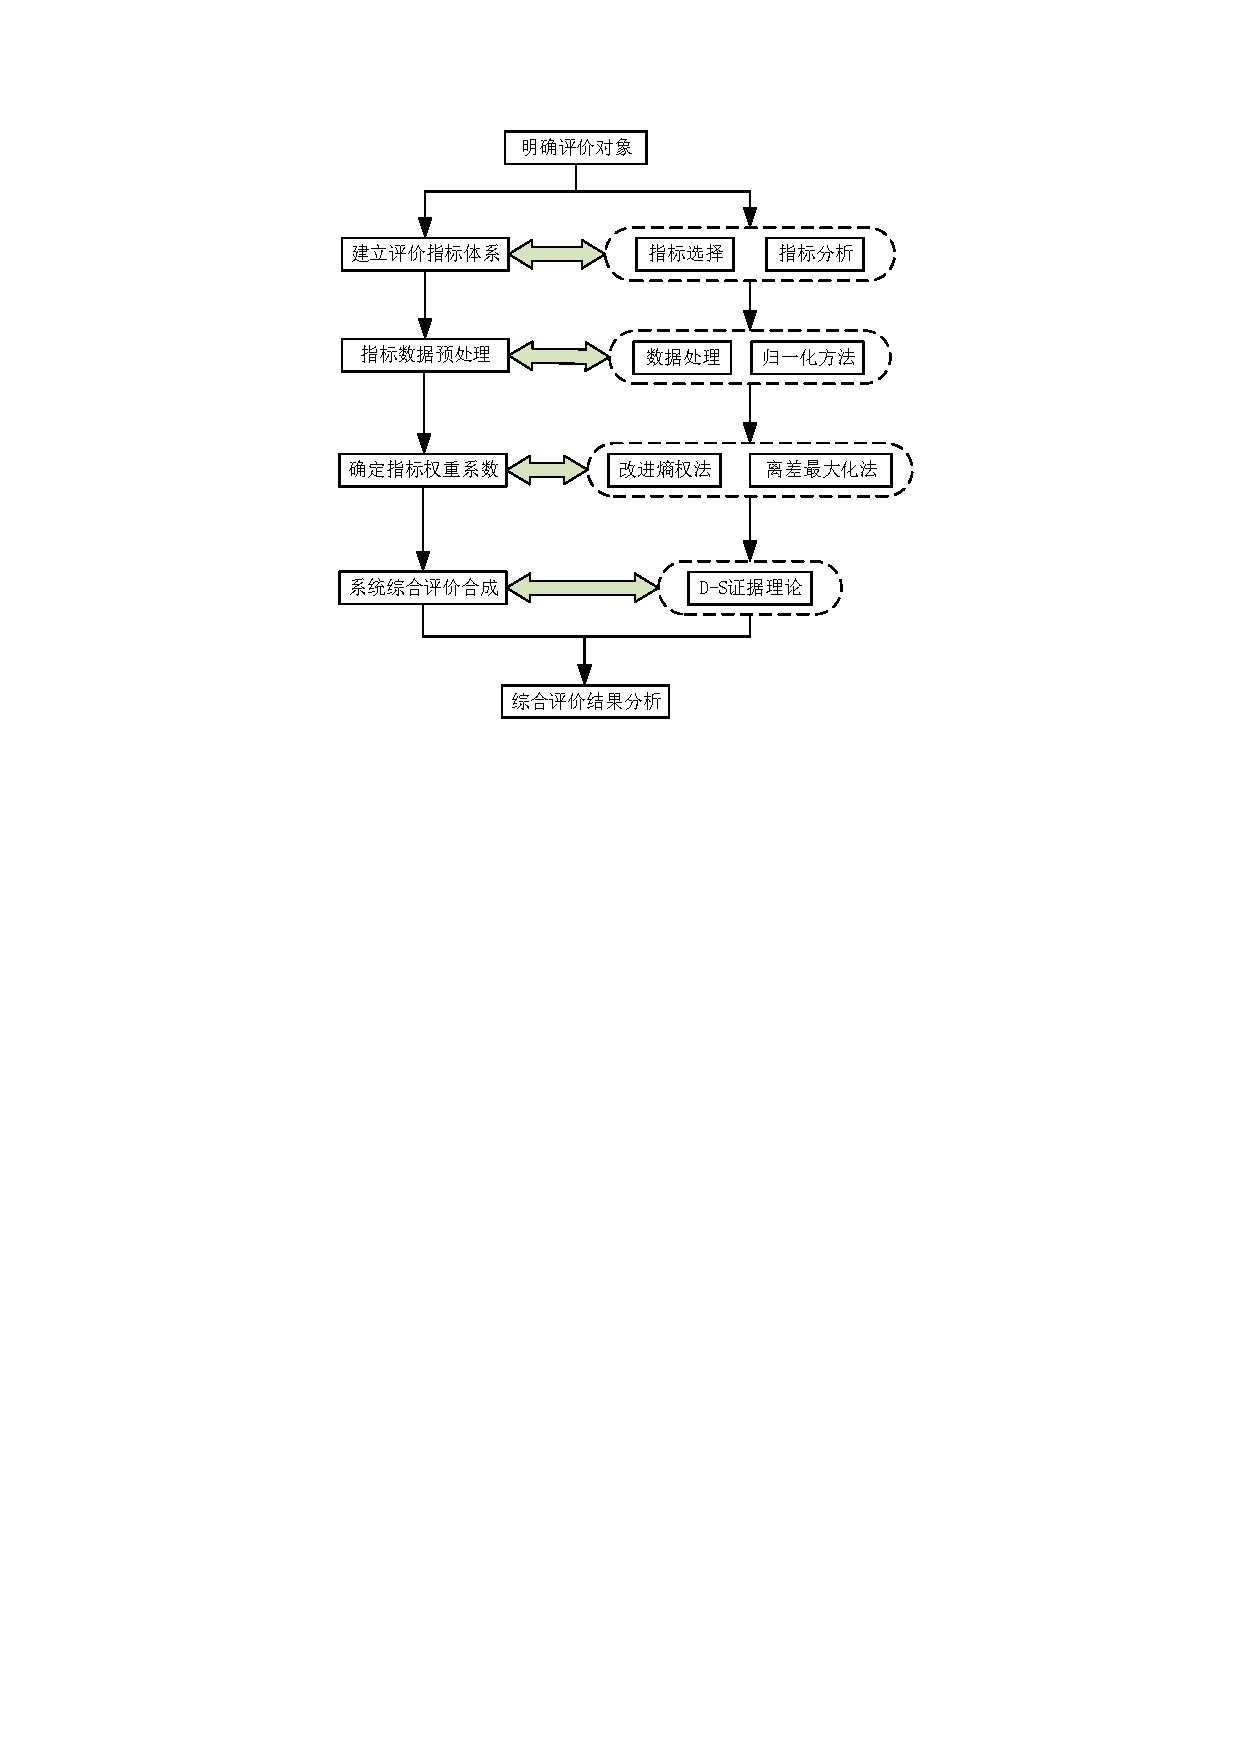
\includegraphics[]{model_procession.pdf}
  \caption{系统脆弱性评价模型流程图}
  \label{fig:model_procession}
\end{figure}


\section{本章小结}
\label{sec:sum4}
本章在系统脆弱性的研究基础上,根据脆弱性的定义与特征,针对结构脆弱性和状态脆弱性分别选取了3个能够反映脆弱性的指标,采用和改进多指标融合方法得到结构脆弱性和状态脆弱性的一级指标。
最后,在$D-S$证据理论的研究基础上,将结构脆弱性指标与状态脆弱性指标进行融合,得到了系统脆弱性综合评价指数,为后文的脆弱性量化分析提供理论基础。



